\documentclass[12pt]{article}
\usepackage{graphicx}
\usepackage{fullpage}
\usepackage{amsmath,enumerate,here}
\usepackage{gensymb}



\begin{document}

\section{Transition Radiation}

The equation for transition radiation can be found in this paper [1]. It can also be found in the Accelerator Handbook [2]. We assume that the electrons travel through a vacuum upon entering the foil with dielectric constant $\epsilon$. In this calculation, we use a dielectric constant of 11.9 for silicon and 250 for titanium metal (titanium in reality is much closer to an ideal conductor). The differential energy d$W$ per electron emitted at an angle $\theta$ from the backwards normal of the foil per solid angle per unit frequency is given by

\begin{equation}
\frac{dW} {d \Omega d \omega} =\frac{e^{2} \beta^{2} \sin^2 \theta \cos^2 \theta} {\pi^{2} c (1-\beta^{2} \cos^2 \theta)^{2}} \times \left( \frac{(\epsilon -1) (1-\beta^{2}+\beta \sqrt{\epsilon-\sin^2 \theta})} {(1+\beta \sqrt{\epsilon-\sin^2 \theta}) (\epsilon \cos \theta + \sqrt{\epsilon- \sin^2 \theta})} \right)^{2}
\end{equation}
where $e$ is the charge of an electron, $c$ is the speed of light, and $\beta$ is the fraction of $c$ that the electrons are traveling. In the limit of a perfect conductor (i.e. $\epsilon \rightarrow \infty$), the equation simplifies to

\begin{equation}
\frac{dW} {d \Omega d \omega} =\frac{e^{2} \beta^{2} \sin^2 \theta} {\pi^{2} c (1-\beta^{2} \cos^2 \theta)^{2}}
\end{equation}

\begin{figure}
\begin{center}
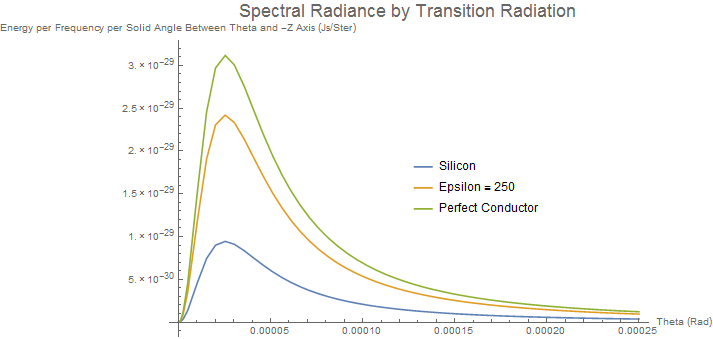
\includegraphics[scale=0.5]{dWdomega.PNG}
\caption{This figure shows the spectral radiance for the transition radiation $\frac{\mathrm{d}W}{\mathrm{d} \omega \mathrm{d} \Omega}$ for angle $\theta$ with respect to the normal of the foil.}
\end{center}
\end{figure}
This is shown in Fig. 1 for silcon, titanium, and a perfect conductor. There is a peak at a maximum of $\frac{1}{\gamma}$. For a non-perfect conductor, integrating over all of $\phi$ and over the $\theta$ that is covered by the camera lens $\theta_a$ is given by

\begin{equation}
\frac{dW} {d \omega} =2 \pi \int\limits_0^{\theta_{a}} \sin \theta \frac{e^{2} \beta^{2} \sin^2 \theta \cos^2 \theta} {\pi^{2} c (1-\beta^{2} \cos^2 \theta)^{2}} \times \left( \frac{(\epsilon -1) (1-\beta^{2}+\beta \sqrt{\epsilon-\sin^2 \theta})} {(1+\beta \sqrt{\epsilon-\sin^2 \theta}) (\epsilon \cos \theta + \sqrt{\epsilon- \sin^2 \theta})} \right)^{2} \mathrm{d} \theta
\end{equation}
Doing the same integration to a perfect conductor gives

\begin{equation}
\frac{dW} {d \omega} =2 \pi \int\limits_0^{\theta_{a}} \sin \theta \frac{e^{2} \beta^{2} \sin^2 \theta} {\pi^{2} c (1-\beta^{2} \cos^2 \theta)^{2}} \mathrm{d} \theta
\end{equation}
This integration for the perfect conductor is done exactly in [2] and gives the following

\begin{equation}
\frac{dW} {d \omega} (\theta_{a}) =\frac{e^{2}} {2 \pi c} \times \left( \frac{2(1-\beta^{2}) \cos \theta_{a}}{1-\beta^2 \cos^2 \theta_{a}}+\frac{1+\beta^{2}}{\beta} \ln{\frac{(1-\beta \cos \theta_{a})(1+\beta)}{(1+\beta \cos \theta_{a})(1-\beta)}}-2 \right)
\end{equation}
where $\theta_a$ is the angle that the camera covers. Assuming that we know the results above, we can now attempt to back out the number of photons emitted in the visible spectrum. Fig. 2 gives the total energy collected by the camera that covers an angle $\theta_a$. Notice that the above equations are independent of frequency, thus each frequency in the visible range emits the same amount of energy. 

\begin{figure}
\begin{center}
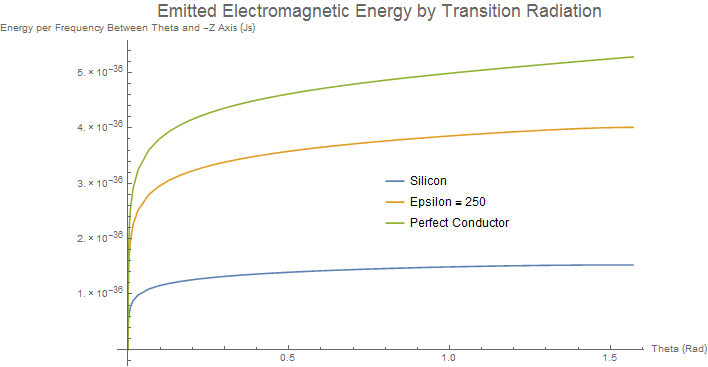
\includegraphics[scale=0.5]{Energy2.PNG}
\caption{This figure shows the total energy per electron collected by the camera that covers an angle $\theta$.}
\end{center}
\end{figure}


\begin{equation}
\mathrm{d} W=n \hbar \mathrm{d} \omega
\end{equation}

\begin{equation}
n=\frac{\mathrm{d} W}{\mathrm{d} \omega} \frac{1}{\hbar}
\end{equation}

\begin{equation}
n_{visible}=\frac{\mathrm{Total Visible Energy}}{\mathrm{Average Energy per Photon}}=\frac{\mathrm{d} W}{\mathrm{d} \omega} \frac{\omega_2 - \omega_1}{\hbar \omega_{avg}}
\end{equation}
The results of the calculation are shown in Fig. 3 for given input parameters such as the distance from the camera to the interaction point $d$, diameter of the lens $a$, $\gamma$, and various dielectric constants $\epsilon$.

\begin{figure}
\begin{center}
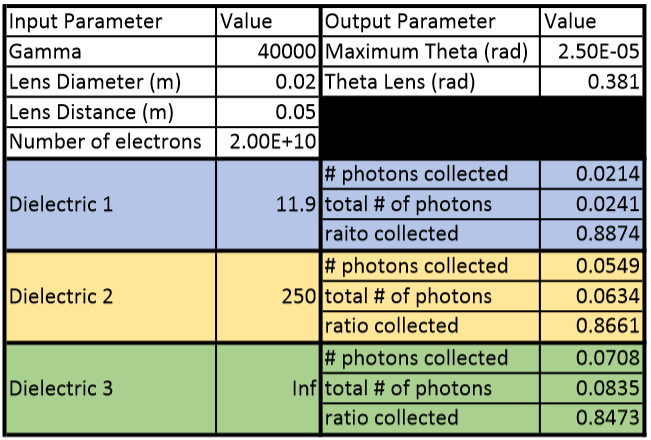
\includegraphics[scale=0.5]{TransData.PNG}
\caption{This table shows the input parameters and various output paramters such as the number of photons emitted by transition radiation (per electron) as well as other relevant parameters.}
\end{center}
\end{figure}

\section{Diffraction Radiation from a Hole}

The diffraction radiation equation can be found in the Accelerator Handbook [2]. This equation applies to a circular hole in a foil, and it is the energy emitted per electron at a distance $r$ from the center of the hole of radius $a$. It is a function of the transition radiation $\frac{dW_{TR}} {d \Omega d \omega}$.

\begin{equation}
\frac{dW} {d \Omega d \omega}=\frac{dW_{TR}} {d \Omega d \omega} [J_{0}(ka \sin \theta)^{2}+(\frac {r}{a})^{2} J_{1}(ka \sin \theta)^{2}]
\end{equation}
where $k=\frac{\omega}{c}$. Thus, the differential diffraction radiation does depend on frequency.

\begin{equation}
\frac{dW} {d \Omega d \omega}=\frac{dW_{TR}} {d \Omega d \omega} [J_{0}(\frac {\omega a}{c} \sin \theta)^{2}+(\frac {r}{a})^{2} J_{1}(\frac {\omega a}{c} \sin \theta)^{2}]
\end{equation}
Integrating around all of d$\phi$ and also d$\theta$ and d$\omega$ gives

\begin{equation}
W(r)= 2 \pi \int_{\omega_{1}}^{\omega_{2}} \int_{0}^{\theta_{a}} \sin \theta \frac{dW_{TR}} {d \Omega d \omega} [J_{0}(\frac {\omega a}{c} \sin \theta)^{2}+(\frac {r}{a})^{2} J_{1}(\frac {\omega a}{c} \sin \theta)^{2}] \mathrm{d} \theta \mathrm{d} \omega
\end{equation}
The energy emitted per electron is a function of $r$, the distance from the center of the hole. Thus, we must know the density of electrons at each point. I will have to look up exactly what the density function for a bunch of particles, but I remember it is some form of a Gaussian. Let's say the density is radially symmetric, $\rho (r)$ and the center of the beam travels in the center of the hole. Then the differential energy from the emitted visible photons at a distance $r$ from the center in the region d$r$ is

\begin{equation}
\mathrm{d}W_{total}(r)=2 \pi \rho (r) W(r) \mathrm{d}r
\end{equation}
Using the equation in the previous section, the number of photons emitted d$n$ at a distance $r$ in s small interval d$r$ is given by

\begin{equation}
\mathrm{d}n=\mathrm{d} W_{total} \frac{1}{\hbar \omega_{avg}}
\end{equation}
Finally, integrating over $r$ gives the total number of photons

\begin{equation}
n=\int_0^{\infty} \mathrm{d} W_{total} \frac{1}{\hbar \omega_{avg}}
\end{equation}
In addition to a hole not being very practical to an experiment, the integration proved too difficult for Mathematica to do accurately so the results are not presented here.


\section{Diffraction Radiation of a Flat Edge}

The spectral intensity $\frac{dI}{d \omega}$ for optical diffraction radiation from a flat metal foil with an impact parameter of $\vec{u}=u_x \hat{i}+u_y \hat{y}$ is found in Lumpkin's paper [4] and is given by

\begin{equation}
\frac{dI}{d \omega}(u_x,u_y,\omega)=\frac{e^2}{\pi^2 c \beta^2} \frac{1}{(\gamma \lambda)^2} \frac{N}{2 \pi \sigma_x \sigma_y} \int \int K_{1}^{2} \left( \frac{1}{\gamma \lambda} \sqrt{(u_x-x)^2+(u_y-y)^2} \right) e^{- \left( \frac{x^2}{2 \sigma_{x}^{2}}+\frac{y^2}{2 \sigma_{y}^{2}} \right) } dx dy
\end{equation}
where $\sigma_x$ and $\sigma_y$ are the beam sizes in the $x$ and $y$ directions, respectively, $N$ is the total number of electrons, $\lambda$ is the wavelength, and $K_1^{2}$ is the modified Bessel function. In the analysis, it is important to analyze both the $x$ and $y$ projections, which are $\frac{dI_x}{d \omega}$ and $\frac{dI_y}{d \omega}$, respectively.

\begin{equation}
\frac{dI_x}{d \omega}(u_x, \omega)=\frac{e^2}{\pi^2 c \beta^2} \frac{1}{(\gamma \lambda)^2} \frac{N}{2 \pi \sigma_x \sigma_y} \int_{u_y=a}^{\infty} \int \int K_{1}^{2} \left( \frac{1}{\gamma \lambda} \sqrt{(u_x-x)^2+(u_y-y)^2} \right) e^{- \left( \frac{x^2}{2 \sigma_{x}^{2}}+\frac{y^2}{2 \sigma_{y}^{2}} \right) } dx dy du_y
\end{equation}
where $a$ is the impact parameter.

\begin{equation}
\frac{dI_y}{d \omega}(u_y,\omega)=\frac{e^2}{\pi^2 c \beta^2} \frac{1}{(\gamma \lambda)^2} \frac{N}{2 \pi \sigma_x \sigma_y} \int \int \int K_{1}^{2} \left( \frac{1}{\gamma \lambda} \sqrt{(u_x-x)^2+(u_y-y)^2} \right) e^{- \left( \frac{x^2}{2 \sigma_{x}^{2}}+\frac{y^2}{2 \sigma_{y}^{2}} \right) } dx dy d_ux
\end{equation}
Also, the total number of visible photons $n$ emitted due to diffraction radiation is given by

\begin{equation}
n=A \int_{\omega_1}^{\omega_2} \int_{a}^{\infty} \int \int \int K_{1}^{2} \left( \frac{1}{\gamma \lambda} \sqrt{(u_x-x)^2+(u_y-y)^2} \right) e^{- \left( \frac{x^2}{2 \sigma_{x}^{2}}+\frac{y^2}{2 \sigma_{y}^{2}} \right) } dx dy du_x du_y d \omega
\end{equation}
where

\begin{equation}
A=\frac{1}{4 \pi \epsilon_0} \frac{e^2}{\pi^2 c \beta^2 \hbar \omega_{avg}} \frac{1}{(\gamma \lambda)^2} \frac{N}{2 \pi \sigma_x \sigma_y}
\end{equation}
where $\omega_1$ and $\omega_2$ are the lower and upper frequencies of visible light, respectively, $\omega_{avg}$ is the average visible frequency, and the factor $\frac{1}{4 \pi \epsilon_0}$ is multiplied to the integral. The results are shown below in the following figures. An important result of the these calculations is that it is very difficult to resolve the small beam sizes using ODR. Fig. 10 shows that there is very little difference between the width of the $x$ intensity for small beam sizes such as 10 $\mu$ m and 20 $\mu$ m beams. The greater the impact parameter of the ODR foil, the more difficult it is to resolve the spot size. In principle, one could decrease the impact parameter, but then one runs the risk of picking up OTR signals by electrons on the outside of the beam. The results show that ODR is a practical beam diagnostic for larger spot sizes, but ODR is not a practical beam diagnostic for smaller spot sizes.

\begin{figure}
\begin{center}
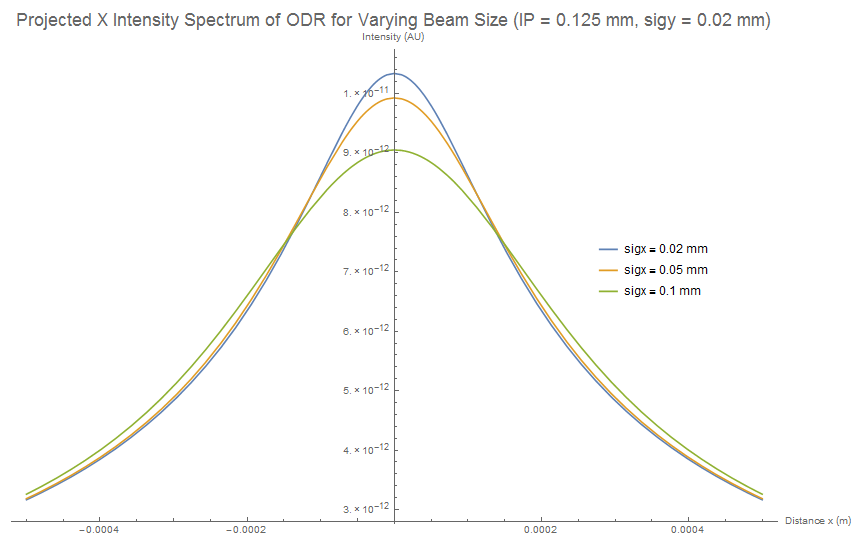
\includegraphics[scale=0.75]{figures/ODR_ProjY_IntensityX.PNG}
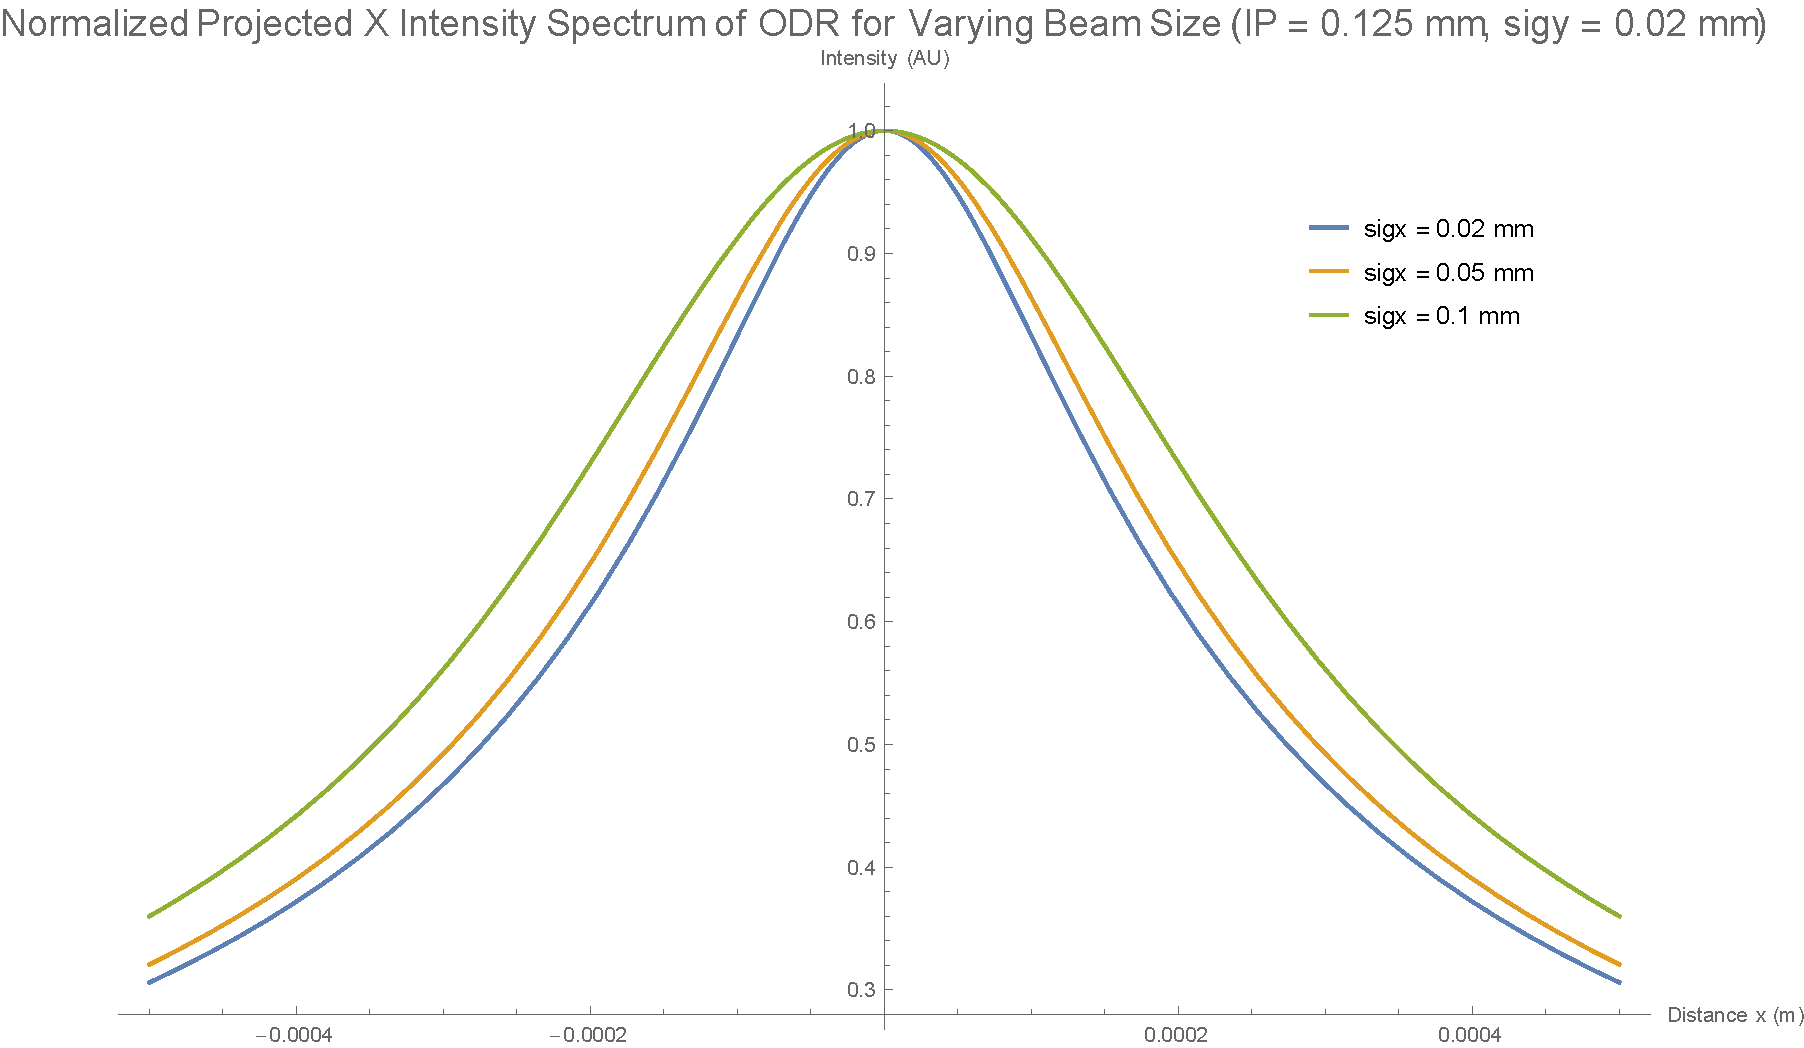
\includegraphics[scale=0.5]{figures/ODR_ProjY_Norm_IntensityX.PDF}
\caption{This figure shows the projected x intensity spectrum (a) and the normalized projected x intensity spectrum (b) for varying x beam size for an impact paramter of 0.125 mm and a y beam size of 20 $\mu m$.}
\end{center}
\end{figure}

\begin{figure}
\begin{center}
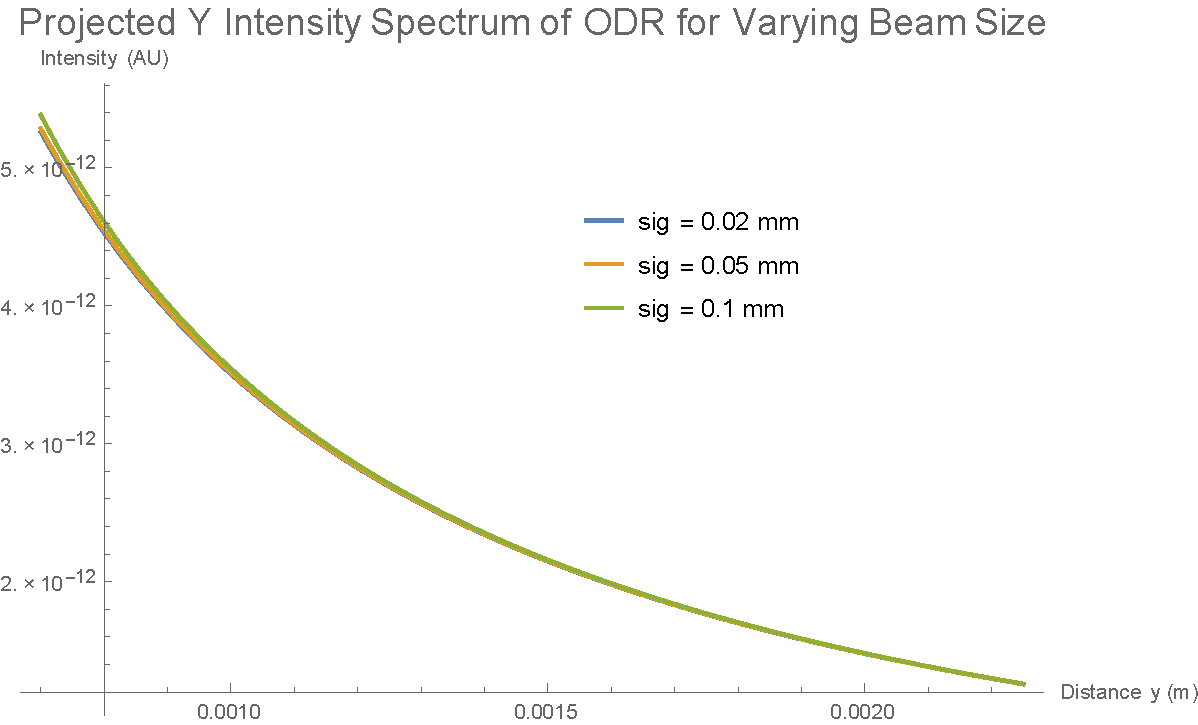
\includegraphics[scale=0.5]{figures/ODR_ProjX_IntensityY.PDF}
\caption{This figure shows the projected y intensity spectrum for varying x beam size for an impact paramter of 0.125 mm and a y beam size of 20 $\mu m$.}
\end{center}
\end{figure}

\begin{figure}
\begin{center}
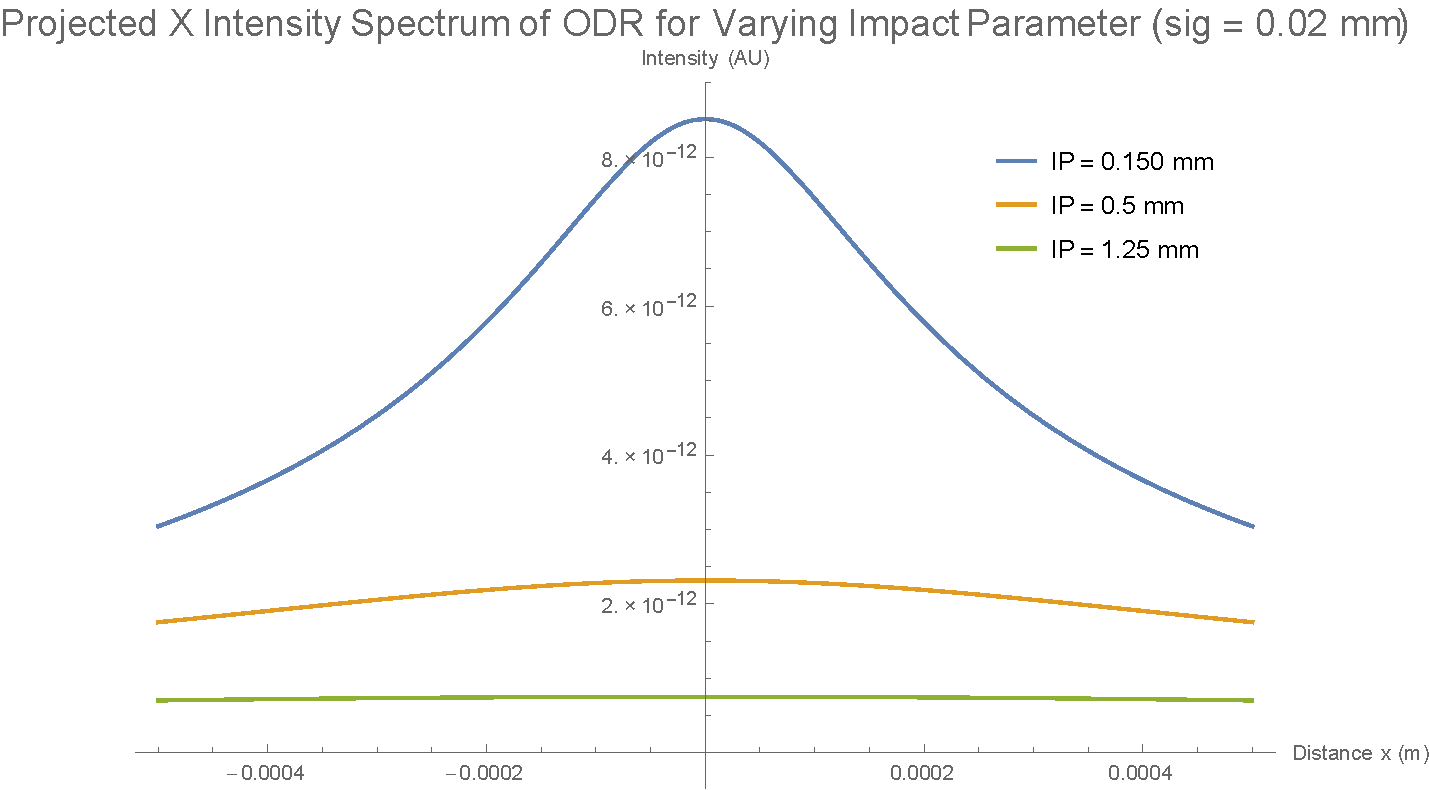
\includegraphics[scale=0.5]{figures/ODR_ProjY_IntensityX_IP.PDF}
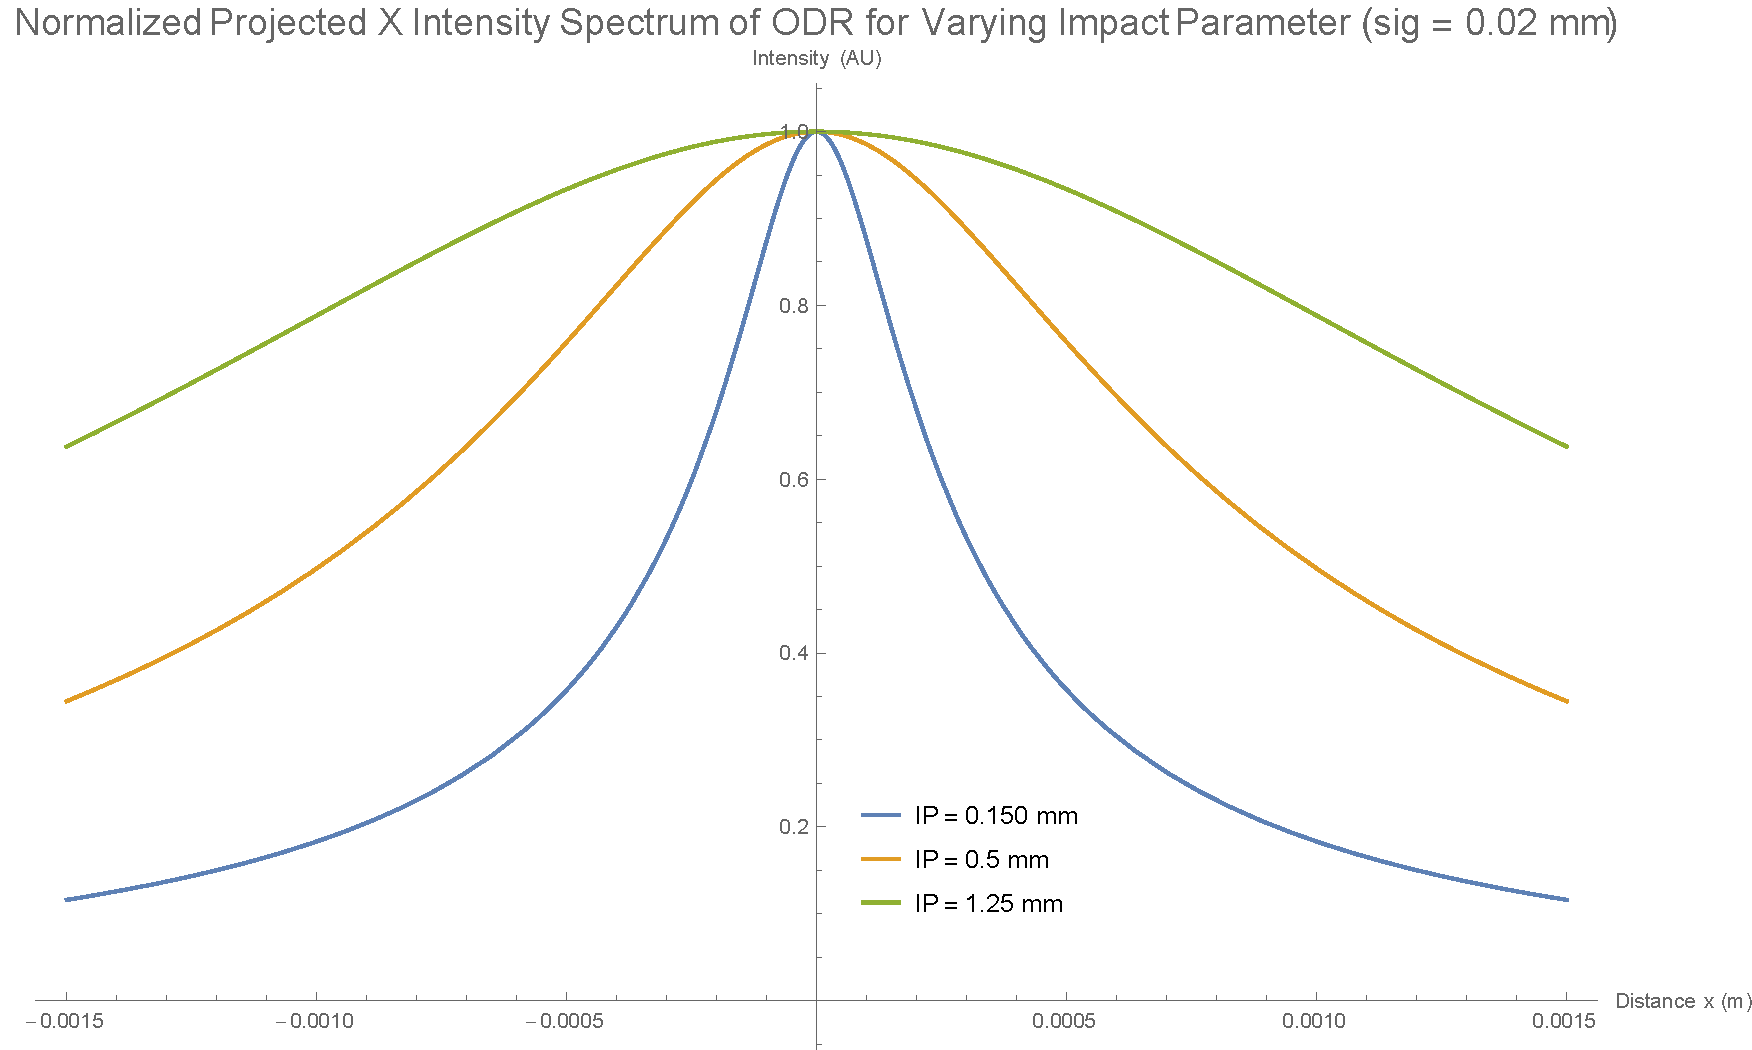
\includegraphics[scale=0.5]{figures/ODR_ProjY_Norm_IntensityX_IP.PDF}
\caption{This figure shows the projected x intensity spectrum (a) and the normalized projected x intensity spectrum (b) for varying impact paramter and a beam size of 20 $\mu m$}
\end{center}
\end{figure}

\begin{figure}
\begin{center}
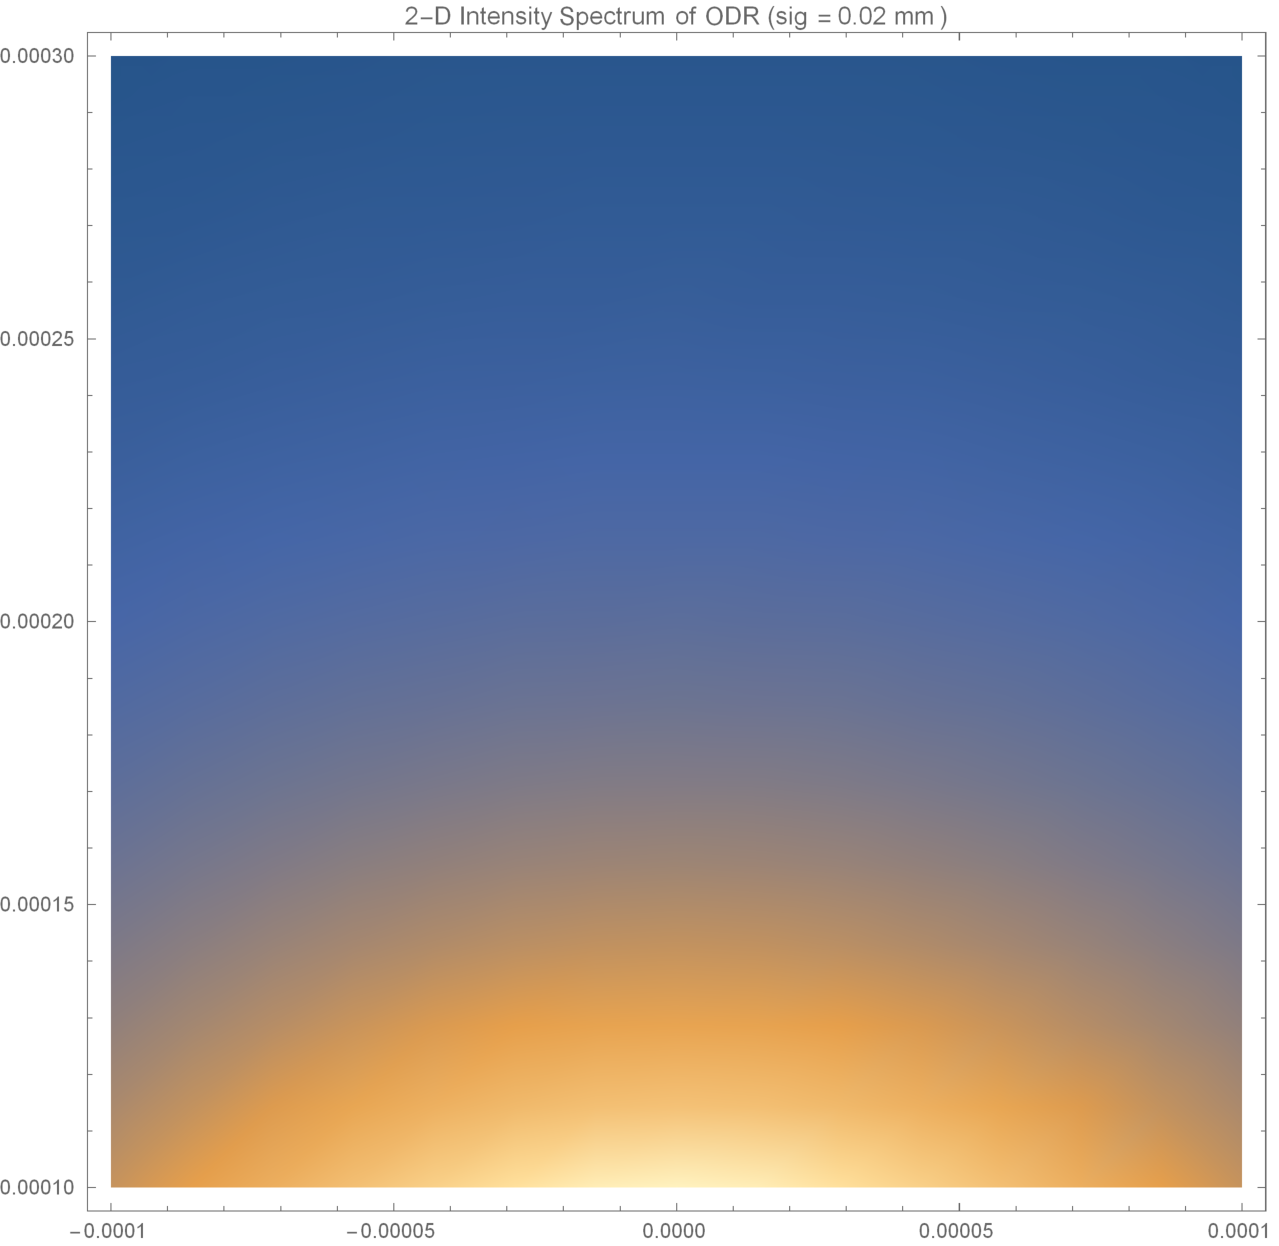
\includegraphics[scale=0.5]{figures/ODR_2D_Intensity.PDF}
\caption{This figure shows the relative 2-D intensity spectrum for a beam size of 20 $mu m$.}
\end{center}
\end{figure}

\begin{figure}
\begin{center}
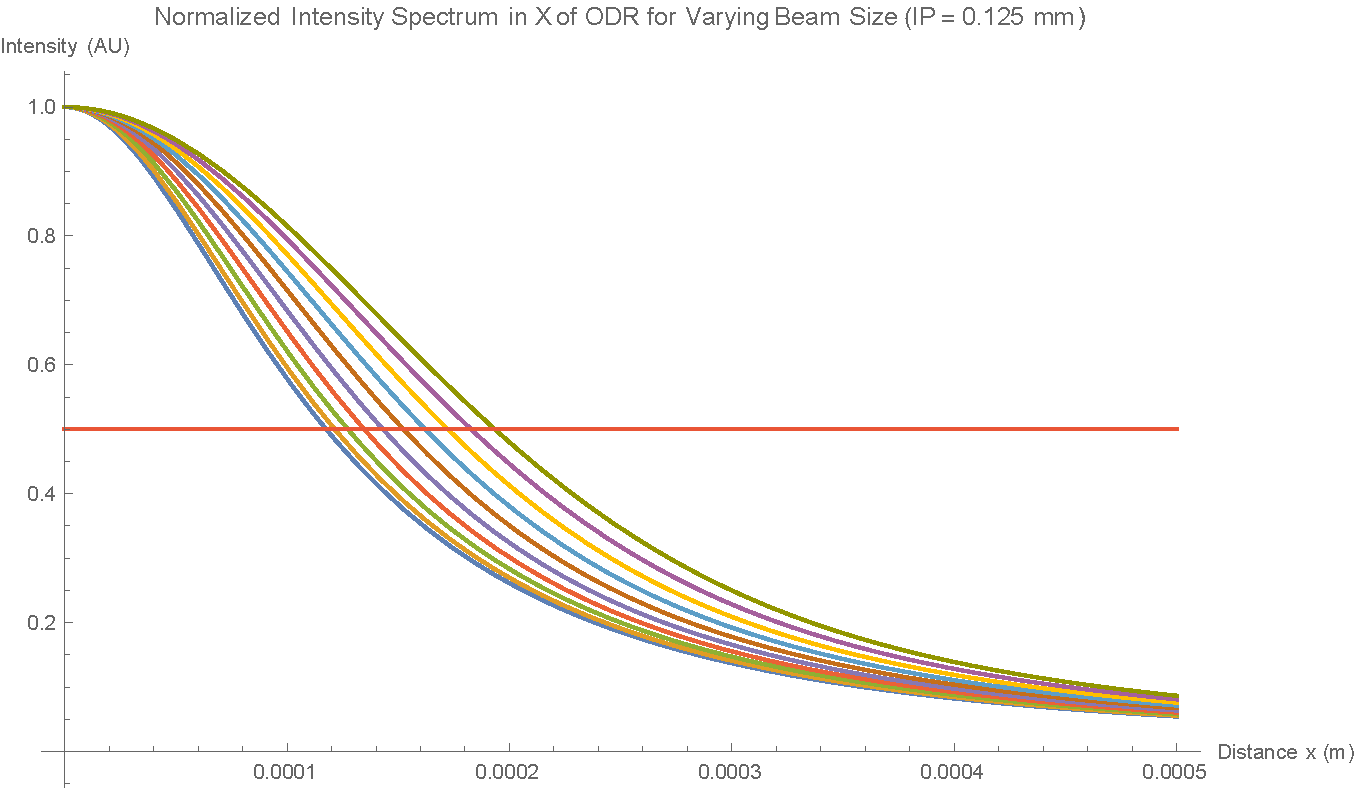
\includegraphics[scale=0.5]{figures/ODR_Norm_IntensityX_125.PDF}
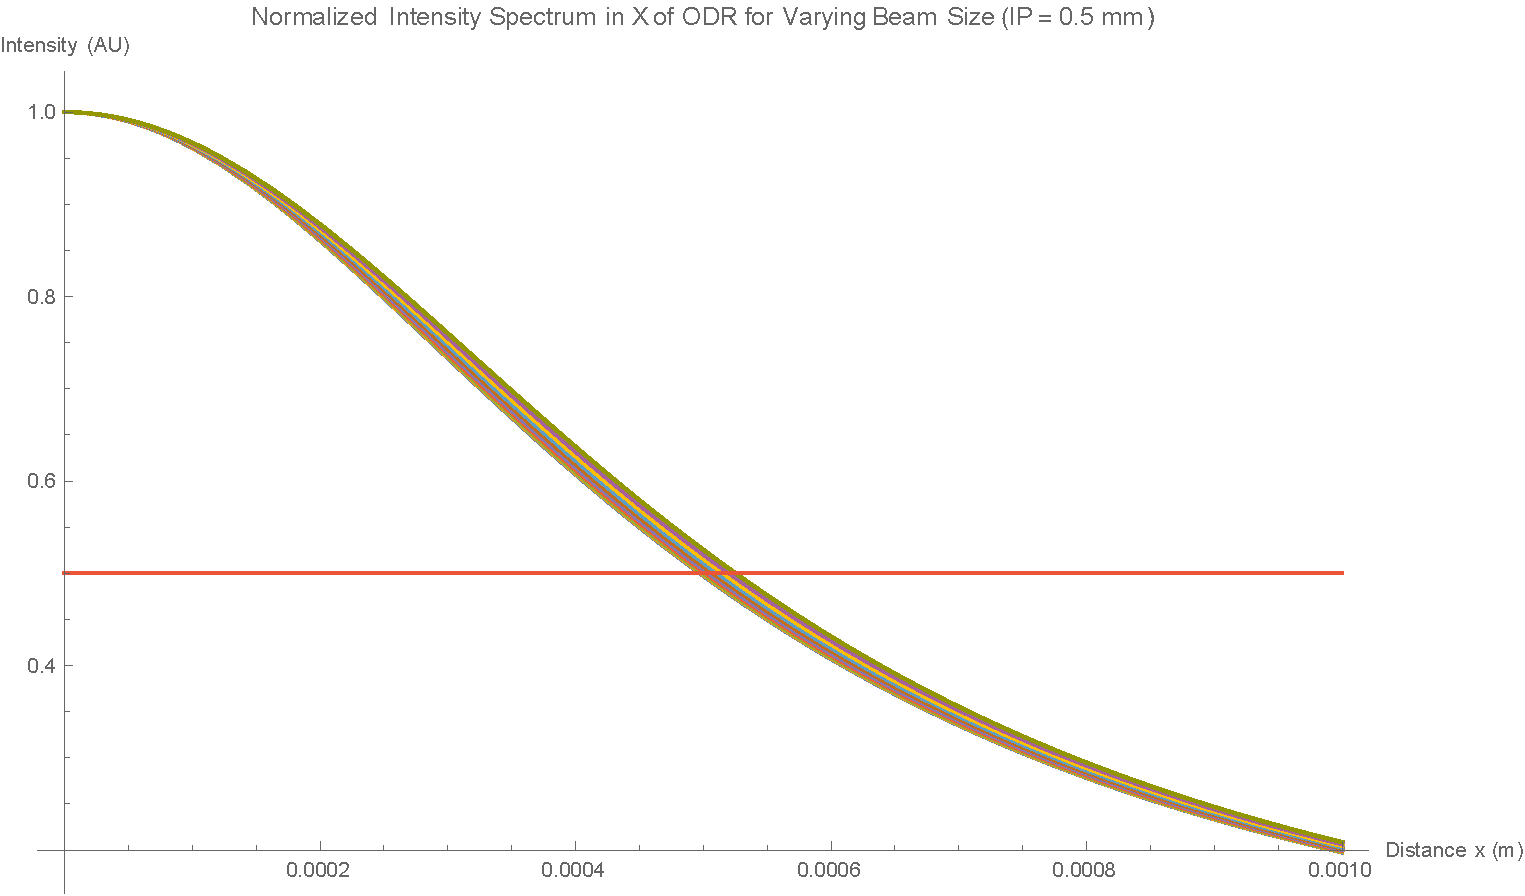
\includegraphics[scale=0.5]{figures/ODR_Norm_IntensityX_500.PDF}
\caption{This figure shows the normalize projected x intensity spectrum for varying x beam size for an impact paramter of 0.125 mm (a) 0.5 mm (b) and and a y beam size of 20 $\mu m$.}
\end{center}
\end{figure}

\begin{figure}
\begin{center}
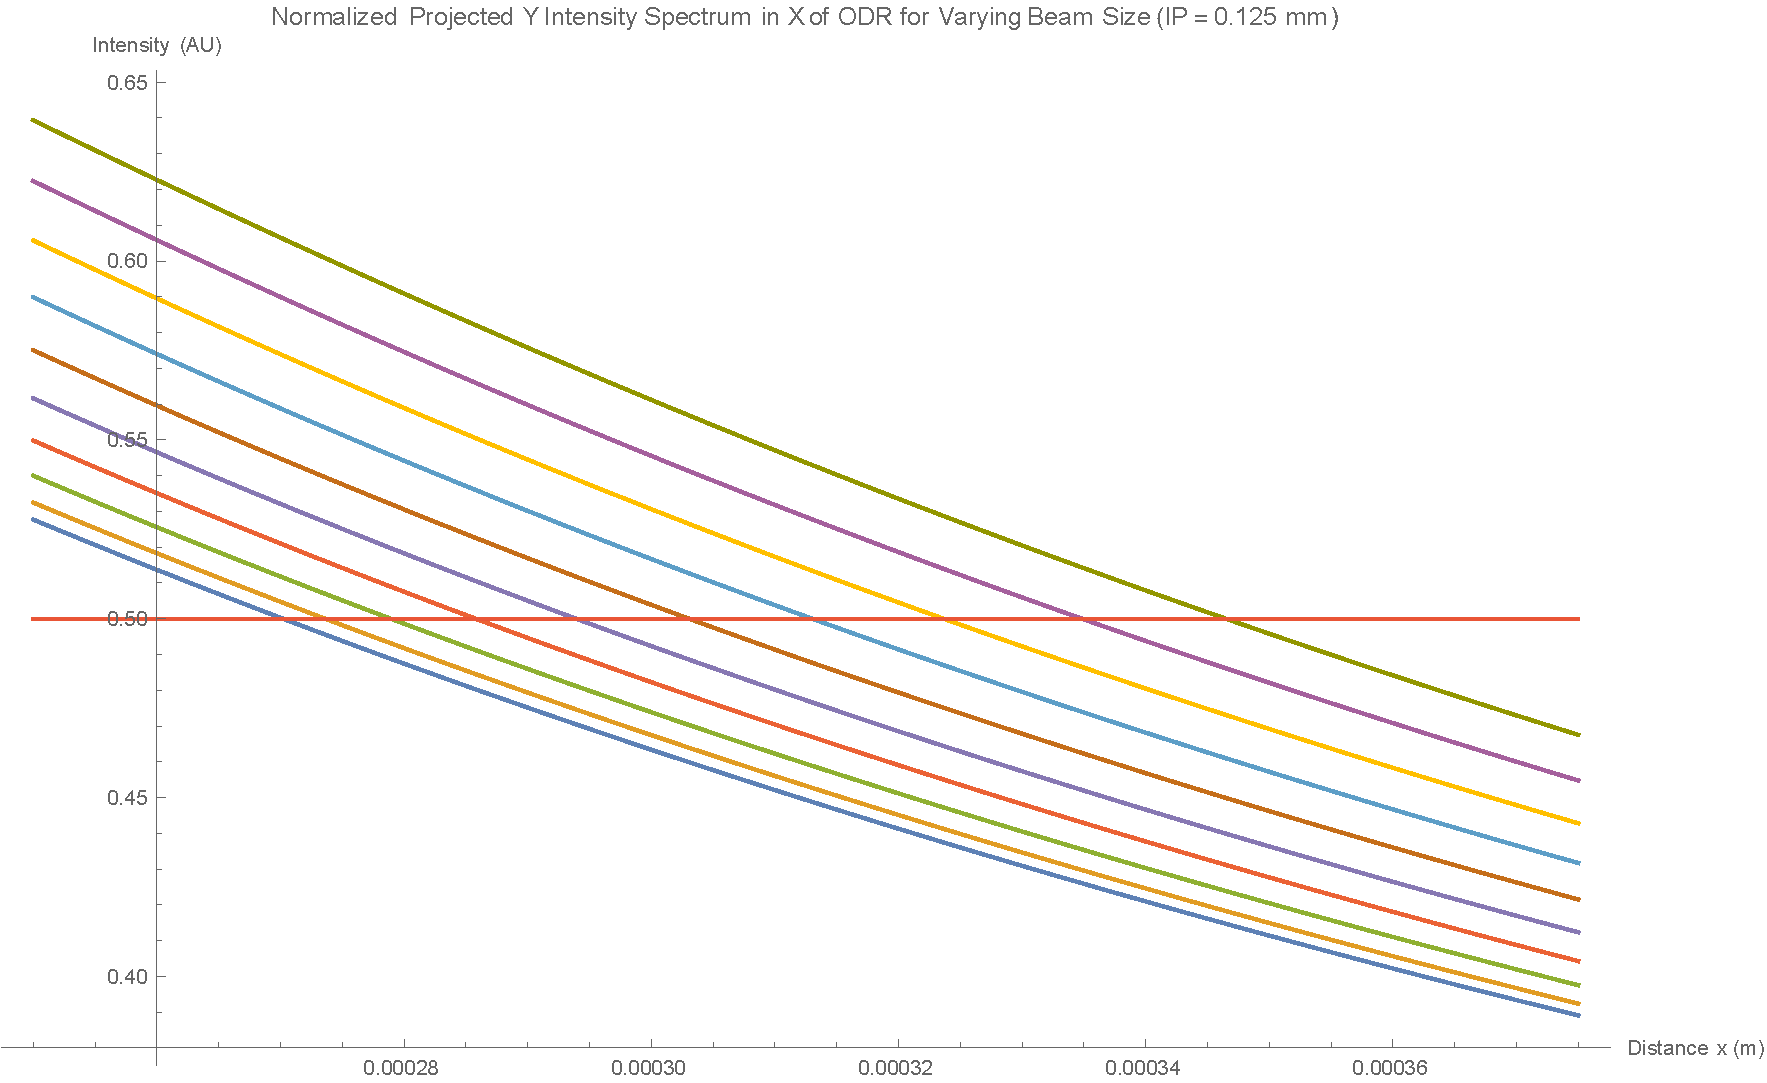
\includegraphics[scale=0.5]{figures/ODR_Norm_ProjY_IntensityX_125_zoom.PDF}
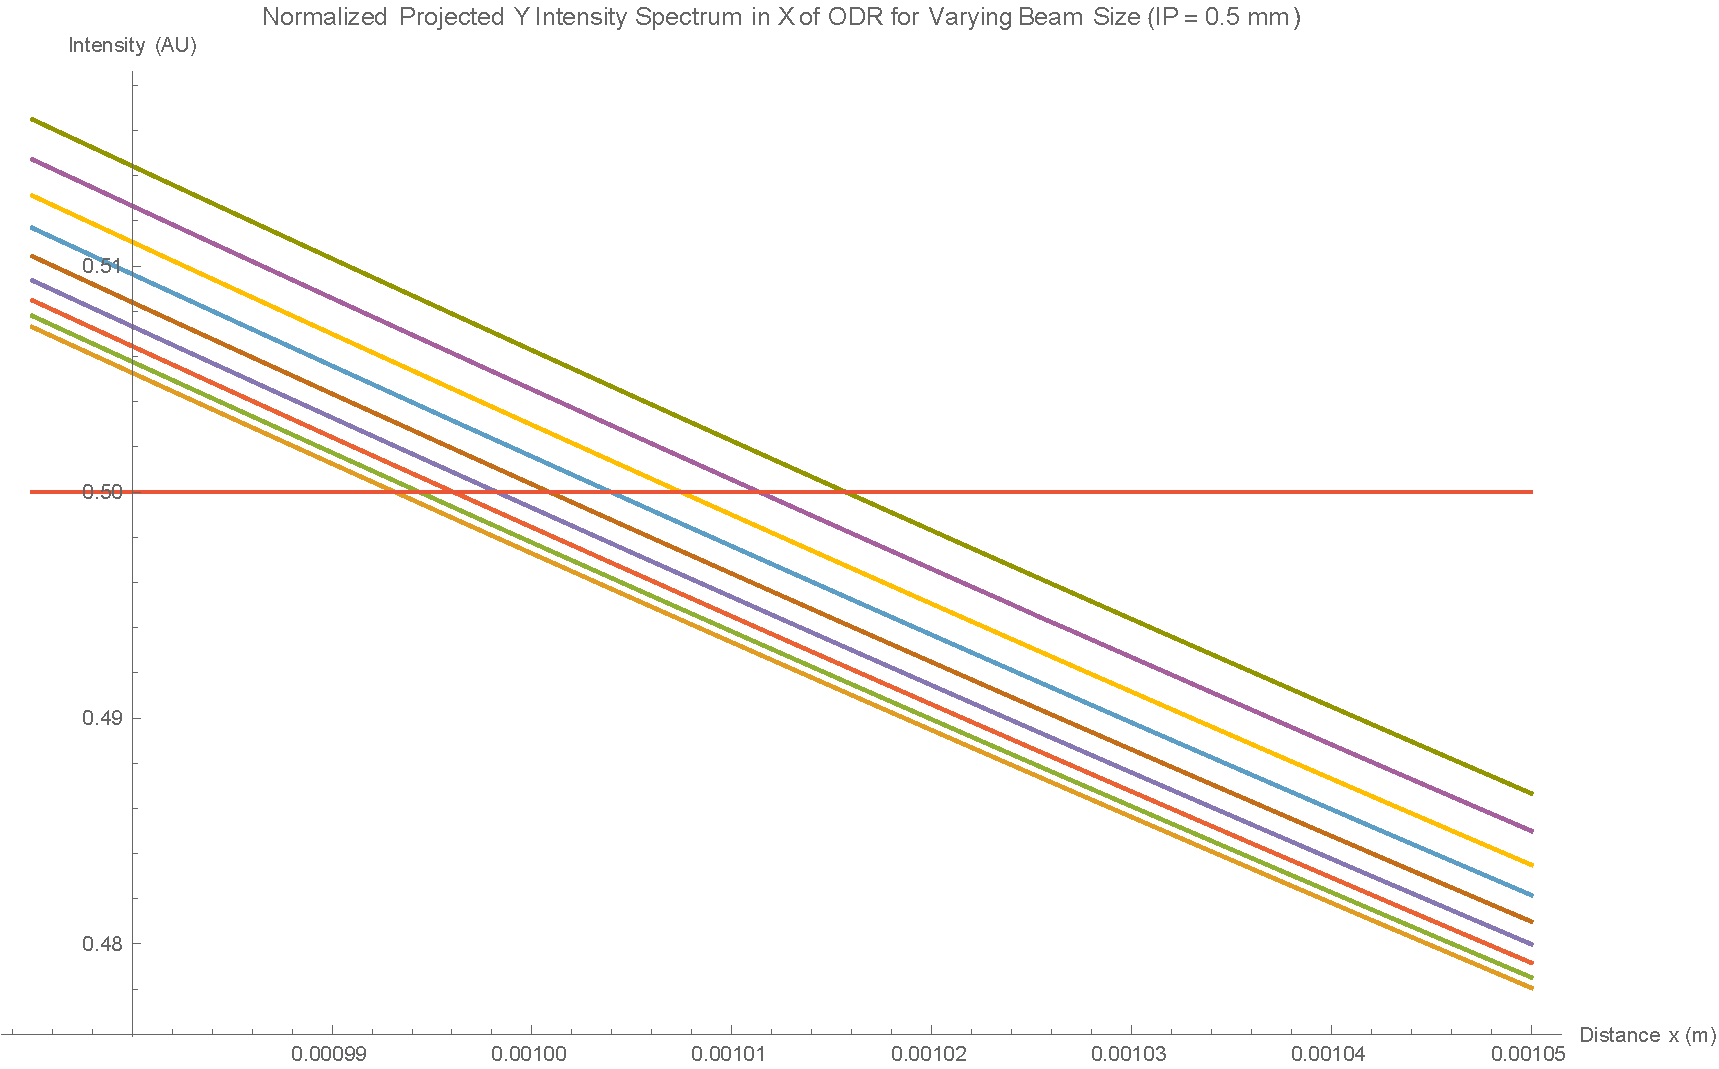
\includegraphics[scale=0.5]{figures/ODR_Norm_ProjY_IntensityX_500_zoom.PDF}
\caption{This figure shows the normalize projected x intensity spectrum for varying x beam size for an impact paramter of 0.125 mm (a) 0.5 mm (b) and and a y beam size of 20 $\mu m$ zoomed in from the previous figure.}
\end{center}
\end{figure}

\begin{figure}
\begin{center}
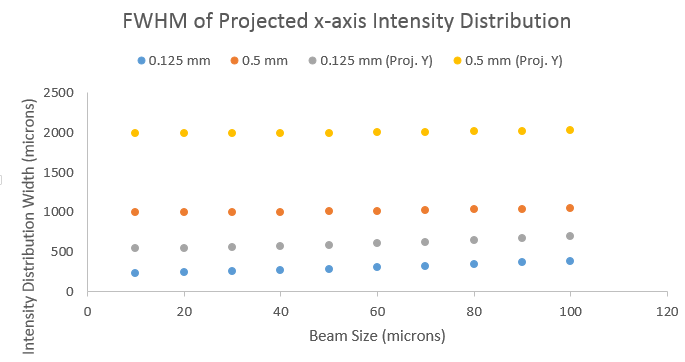
\includegraphics[scale=0.5]{figures/FWHM.PNG}
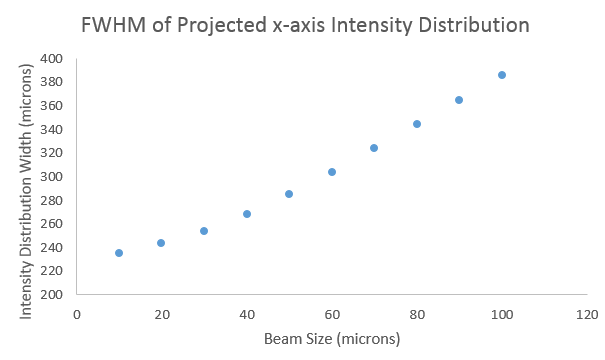
\includegraphics[scale=0.5]{figures/FWHM_125.PNG}
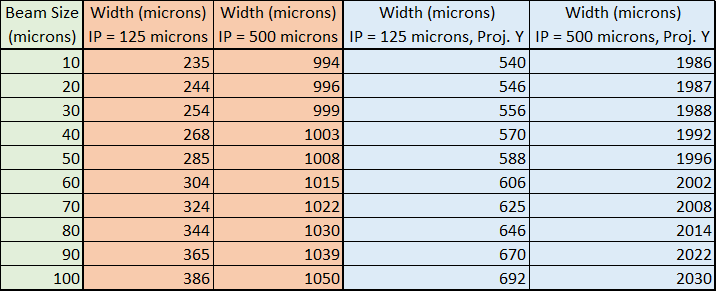
\includegraphics[scale=0.5]{figures/FWHM_Table.PNG}
\caption{This figure shows the full width at half maximum (FWHM) of the measured beam size versus the actual beam size. (a) shows this plot for impact parameters of 0.125 mm and 0.5 mm for both the projected and non-projected intenisities. (b) shows a more detail view of an impact parameter of 0.125 mm. (c) shows a table of the calculated data points.}
\end{center}
\end{figure}




\section{Thermal Radiation - Energy Deposited}

Stupakov's equation for the amount of energy $P$ deposited by a beam in a foil can be found in his paper [3]. In these equations, $Q$ is the total charge of the bunch, $X$ and $Y$ are the dimensionless coordinates $X=\frac{x}{\sigma_z}$ and $Y=\frac{y}{\sigma_z}$, respectively, and $s_x$ and $s_y$ are the dimensionless beam sizes $s_x=\frac{\sigma_x}{\sigma_z}$ and $s_y=\frac{\sigma_y}{\sigma_z}$, respectively. Also, $\Omega=\frac{\omega \sigma_z}{c}$ and $\rho$ is the radius. I am unsure what $\omega$ is, it appears to be the constant of integration when the author does Fourier Transforms. We start with the equation for energy at given coordinates $X$ and $Y$ from the center of the interaction point.

\begin{equation}
P=\frac{Q^2}{4 \pi^{3} \sigma_{x}^{2} \sigma_{y}^{2}} H(X,Y,\Omega,s_x,s_y)
\end{equation}
where

\begin{equation}
H(X,Y,\Omega,s_x,s_y)=\int_0^{\infty} \Omega \mathrm{d} \Omega [|R_{x} (X,Y,\Omega,s_x,s_y)|^2+|R_{y} (X,Y,\Omega,s_x,s_y)|^2]
\end{equation}
where

\begin{equation}
R_{x} (X,Y,\Omega,s_x,s_y)=- \int \mathrm{d} \rho \mathrm{d} \phi \sin \phi \exp{(-\frac{(X+\rho \cos \phi)^2}{2 s_{x}^{2}}-\frac{(Y+\rho \sin \phi)^2}{2 s_{y}^{2}}-\frac{\Omega^2}{2}+i \Omega \rho)}
\end{equation}
and

\begin{equation}
R_{y} (X,Y,\Omega,s_x,s_y)= \int \mathrm{d} \rho \mathrm{d} \phi \cos \phi \exp{(-\frac{(X+\rho \cos \phi)^2}{2 s_{x}^{2}}-\frac{(Y+\rho \sin \phi)^2}{2 s_{y}^{2}}-\frac{\Omega^2}{2}+i \Omega \rho)}
\end{equation}
The temperature change associated with the energy $P$ at each coordinate is given by the simple formula

\begin{equation}
P=k \times m \times \Delta T=k \times m \times (T(X,Y)-T_0)
\end{equation}
where $k$ is the thermal constant of the material, $m$ is the mass, $T(X,Y)$ is the temperature as a function of position on the foil and $T_0$ is the room temperature. Each small element of mass d$m$ will receive a small amount of energy d$P$.

\begin{equation}
\mathrm{d}P=k \mathrm{d}m (T(X,Y)-T_0)
\end{equation}
Solving for $T=T(X,Y)$ gives

\begin{equation}
T=T_0+\frac{1}{k} \frac{\mathrm{d}P}{\mathrm{d}m}=T_0+\frac{1}{k \rho_0} \frac{\mathrm{d}P}{\mathrm{d}V}=T_0+\frac{1}{k \rho_0 d_0} \frac{\mathrm{d}P}{\mathrm{d}A}=T_0+\frac{1}{k \rho_0 d_0} \frac{\mathrm{d}P}{\mathrm{d}X \mathrm{d}Y}
\end{equation}
where $\rho_0$ is the material density and $d_0$ is the skin depth.

The differential of intensity $I$ (energy per time) per solid angle per area per wavelength is given by

\begin{equation}
\frac{\mathrm{d}I}{\mathrm{d} \Omega \mathrm{d}A \mathrm{d} \lambda}=\frac{2hc^2}{\lambda^5} \frac{1}{\exp{\frac{hc}{k_b T}}-1}
\end{equation}
After integrating over $\phi$ for the full 2$\pi$ radians, we can integrate over $\theta$ with the range that the camera covers $\theta_a$ and over the visible spectrum.

\begin{equation}
\frac{\mathrm{d}I}{\mathrm{d}A}=2 \pi \int_{\lambda_1}^{\lambda_2} \int_0^{\theta_a} \sin \theta \frac{\mathrm{d}I}{\mathrm{d} \theta \mathrm{d} \lambda} \mathrm{d} \theta \mathrm{d} \lambda
\end{equation}
We can integrate this function over the entire area.

\begin{equation}
I=\int_{-\infty}^{\infty} \int_{-\infty}^{\infty} \frac{\mathrm{d}I}{\mathrm{d}A} \mathrm{d}X \mathrm{d}Y
\end{equation}
Thus we have the energy per unit time. Finally, we can find the number of photons $n$ per unit time simply by differentiating $E=\frac{hc}{\lambda} n$ and using the average wavelength $\lambda_{avg}$.

\begin{equation}
\frac{\mathrm{d}n}{\mathrm{d}t}=\frac{\lambda_{avg}}{hc} I
\end{equation}
Thus we have the photon rate. Mathematica has difficulty solving these integrals numerically while remaining accurate, so I will simplify the problem to produce usable results.

\section{Thermal Radiation - Steady State}

I will first simplify the problem by analyzing the steady state solution. I will assume steady power distribution to a small spot about the size of a beam. The total power $P$ delivered to the foil from the beam is given by the following equation where we assume a worst case scenario of a foil of thickness $\delta=25 \mu m$.

\begin{equation}
P=-\rho \frac{\mathrm{d} E}{\mathrm{d} x} \times N \times PRR \times \delta
\end{equation}
where $-\rho \frac{\mathrm{d} E}{\mathrm{d} x}$ is the energy loss of an electron per unit length of the foil, $N$ is the number of electrons in the bunch, and $PRR$ is the pulse repititon rate. Plugging in numbers for titanium gives the amount of power delivered over the small area of the foil.

\begin{equation}
P_{Ti}=7.17 \times 10^6 \frac{eV}{cm} \times 10^{10} \times 10 Hz \times 25 \times 10^{-4} cm \times \frac{1.6 \times 10^{-19} J}{1 eV}=0.0002868 W
\end{equation}
The amount of power per unit volume, assuming a beam size of $ \sigma = 25 \mu m$, is

\begin{equation}
S=\frac{P}{V}
\end{equation}
and for the titanium is

\begin{equation}
S_{Ti}=\frac{0.0002868 W}{\pi (20 \times 10^{-4})^2 \times 25 \times 10^{-4} cm^3}=9129 W/cm^3
\end{equation}
We will now compare the power input into the foil with the power radiated away due to temperature differences between the foil $T_1$ and the surroundings $T_2=300 K$.

\begin{equation}
q''_r=\epsilon \sigma (T_{1}^{4}-T_{2}^{4})
\end{equation}
where $\sigma$ is the Stefan-Boltzmann constant, $\epsilon$ is the emissivity of the foil, and $q''_r$ is the power emitted per unit area. For this analysis, we will assume that the foil is $50 \degree C$ below its melting point to obtain a worst case scenario. For titanium, this gives

\begin{equation}
q''_{r Ti}=0.2 \times 5.77 \times 10^{-12} (1900^{4}-300^{4})=15.03 W/cm^2
\end{equation}
And multiplying by the area gives

\begin{equation}
A=\pi \sigma^{2}=\pi (20 \times 10^{-4})^2=1.257 \times 10^{-5} cm^2
\end{equation}

\begin{equation}
P_{r Ti}=q''_{r Ti} \times A=0.000189 W
\end{equation}
Since the power radiated away is much less than the power deposited by the beam, most of the energy must be conducted away. We can start by searching for a steady-state solution to this problem assuming constant power being deilvered to the foil and no radiative heat loss. The difference in temperature between the foil $T_o$ and and the surroundings $T_i$ is given by

\begin{equation}
T_o-T_i=\frac{S \sigma^{2}}{4 K}
\end{equation}
where $k$ is the thermal conductivity of the foil. For titanium, this gives

\begin{equation}
(T_o-T_i)_{Ti}=\frac{9129 W/cm^3 (20 \times 10^{-4})^{2}}{4 \times 0.219 W/cm K}=0.0417 K
\end{equation}
Next, we can find the steady-state temperature difference $\Delta T$ (again assuming no radiative heat loss) between the spot where the beam deposits its energy and the remainder of the foil. We will also assume that the foil has a radius of $r_o=1.27 cm$. 

\begin{equation}
\Delta T=P' \frac{ln(\frac{r_o}{\sigma})}{2 \pi k}
\end{equation}
For titanium, this gives

\begin{equation}
\Delta T_{Ti}=\frac{0.0002868}{25 \times 10^{-6}} W/m \frac{ln(\frac{1.27 cm}{20 \times 10^{-4} cm})}{2 \pi 21.9 W/mk}=0.538 K
\end{equation}
Repeating the method for silicon after gives the following results

\begin{equation}
P_{Si}= 0.000155 W, q''_{r Si}=26.77 W/cm^2 , P_{r Si}=0.000337 W , (T_o-T_i)_{Si}=0.00334 K , \Delta T_{Si}=0.0430 K
\end{equation}
As one can see, the steady-state temperature of both the foil and the spot where the beam deposits its energy is barely above the ambient temperature. Thus, there is no significant visible thermal radiation emitted during steady state.

Now, in order to find the temperature profile as a function of $r$ and $t$, we use the heat equation for radial symmetry. We are assuming only conduction (without thermal radiation) in order to simplify the equation and to provide an upper bound.

\begin{equation}
\rho c_p \frac{\partial T}{\partial t}=\frac{1}{r} \frac{\partial}{\partial r} \left( k r \frac{\partial T}{\partial r} \right)
\end{equation}
where $\rho$ is the density, $c_p$ is the specific heat, and $k$ is the thermal conductivity. The general solution to this equation is as follows.

\begin{equation}
T(r,t)=Ae^{-\alpha t} \left( c_1 J_0 \left( \sqrt{\frac{\alpha \rho c_p}{k}}r \right)+c_2 Y_0 \left( \sqrt{\frac{\alpha \rho c_p}{k}}r \right) \right)
\end{equation}
where $J_0$ and $Y_0$ are Bessel function of the first and second kind, respectively, and $A$, $c_1$, and $c_2$ are arbitrary constants and $\alpha$ is related to how quickly the temperature decreases due to conduction. We must solve the equation for the following boundary conditions

\begin{equation}
T(0 \le r \le \sigma,0)=T_h, T(0,a)=T_0
\end{equation}
where $\sigma$ is the spot size of the beam, $T_h$ is the temperature immediately after the beam deposits energy into the foil, $a$ is the radius of the foil, and $T_0$ is the boundary temperature. To solve this would be a fun academic exercise.

\section{Thermal Radiation - Visible Photons}

In order to efficiently calculate the number of photons (or intensity) emitted due to a heated foil, we must make several assumptions. The most major assumption is that no conduction is present, i.e. the thermal radiation process is too quick for conduction to have effect. Second, the heated foil is only in a circle that is the same area as the cross-sectional area of the beam. Lastly, the foil heats to just below its melting point (50 $\degree$ in this calculation). These three assumptions are the "worst case scenario" and provide an upper bound to the problem. In this calculation, the relevant parameters used are the foil thickness ($\delta=25 \mu m$) and the beam size ($\sigma_r = 20 \mu m$). Calculations were carried out for both titaniu and silicon. We begin the calulation by relating energy $E$ to the temperature $T$ and the nominal temperature $T_0$.

\begin{equation}
E=V \rho c_p (T-T_0)
\end{equation}
where $\rho$ is the material density and $c_p$ is the specific heat of the material. Taking the time derivative gives the power $P$ in terms of the rate of change of temperature.

\begin{equation}
P=\frac{dE}{dt}=V \rho c_p \frac{dT}{dt}
\end{equation}
We also know that the total power given off by thermal radiation is simply the Stephen-Boltzmann Law.

\begin{equation}
P=-2 A \sigma \epsilon T^4
\end{equation}
where $A$ is the area of the heated portion of the foil, $\sigma$ is the Stephan-Boltzmann constant, and $\epsilon$ is the emissivity of the material. Since we are only considering radiation effects, we can set the equations equal to each other and obtain the following differential equation.

\begin{equation}
\frac{dT}{dt}=-\frac{2 A \sigma \epsilon}{V \rho c_p} (T^4-T_{0}^{4})=-\frac{2 \sigma \epsilon}{\delta \rho c_p} (T^4-T_{0}^{4})
\end{equation}
Notice that $\frac{A}{V}=\frac{A}{A \delta}=\frac{1}{\delta}$. Solving the differential equation is done simply by separation of variables, and integrating the temperature from the hottest temperature $T_h$ to $T$ and the time from $0$ to $t$ gives

\begin{equation}
ln \left(\frac{T-T_0}{T+T_0} \right)-2tan^{-1} \left(\frac{T}{T_0} \right)=-(At+C)
\end{equation}
where

\begin{equation}
A=\frac{8T_{0}^{3} \epsilon \sigma}{\delta \rho c_p}, C=ln \left(\frac{T_h+T_0}{T_h-T_0} \right)+2tan^{-1} \left(\frac{T_h}{T_0} \right)
\end{equation}
Unfortunately, we can only obtain an implicit function of $T$. However, since we only care about the case in which $T^4>>T_{0}^{4}$, the case where visible thermal radiation is dominant, we can neglect the $\sigma T_{0}^{4}$ term. This approximation is sufficient because of the 4th power temperature dependence, thus the differential equation reduces to the following.

\begin{equation}
\frac{dT}{dt}=-\frac{2 \sigma \epsilon}{\delta \rho c_p} T^4
\end{equation}

\begin{equation}
\int_{T_h}^{T} \frac{dT'}{T'^4}=\int_0^t -\frac{2 \epsilon \sigma}{\delta \rho c_p} dt'
\end{equation}
This yields the temperature as a function of time. The results for titanium and silicon are shown in the plot.

\begin{equation}
T(t)=T_h \left( 1+\frac{6 \epsilon \sigma}{\delta \rho c_p} T_{h}^{3} t \right)^{-\frac{1}{3}}
\end{equation}

\begin{figure}
\begin{center}
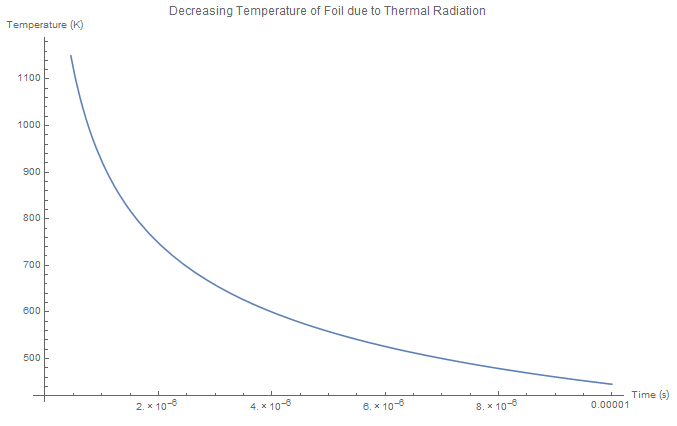
\includegraphics[scale=0.5]{figures/TemperatureTi.PDF}
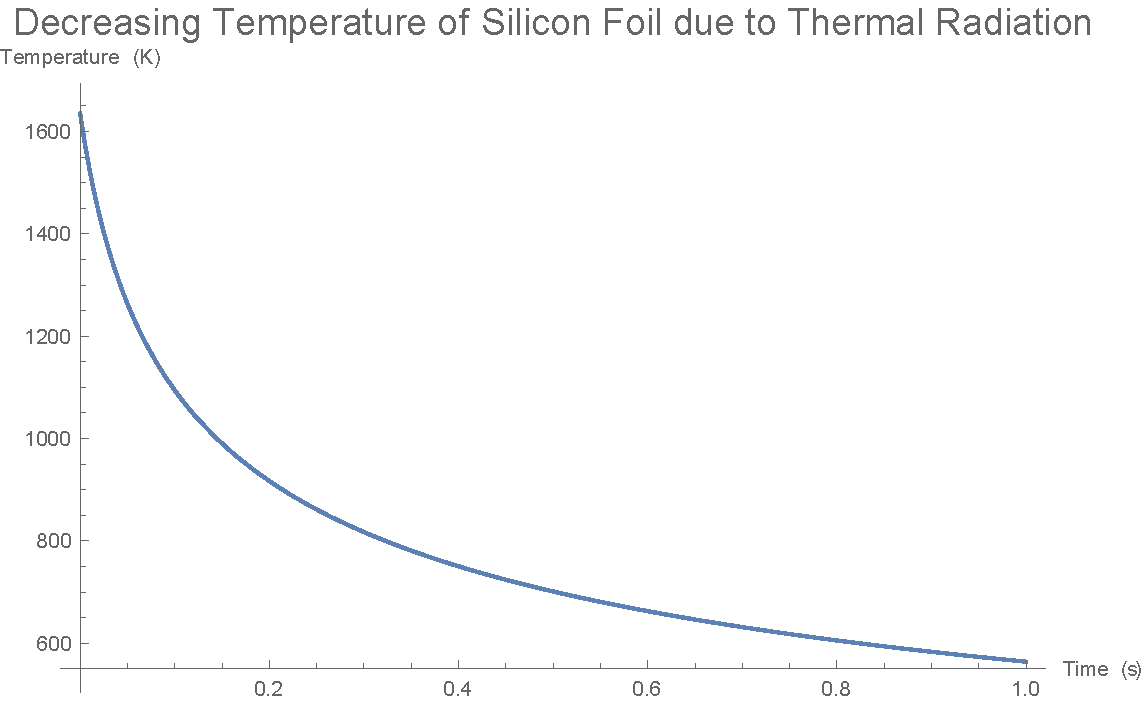
\includegraphics[scale=0.5]{figures/TemperatureSi.PDF}
\caption{This figure shows the temperature of the foil as a function of time for both titanium (a) and silicon (b). This neglects effects due to conduction.}
\end{center}
\end{figure}
In order to find the number of photons emitted, we start with blackbody radiation which gives the energy per area per solid angle per wavelength per time.

\begin{equation}
\frac{dE}{dA d \Omega dt d \lambda} = \frac{2 h c^2}{\lambda^{5}} \frac{1}{e^{\frac{hc}{\lambda k_B T}}-1}
\end{equation}
where $\Omega$ is the solid angle, $\lambda$ is the wavelength, $h$ is Planck's constant, $c$ is the speed of light, and $k_B$ is Boltzmann's constant. We can easily integrate over area ($A=\pi \sigma_r^2$) which is constant and the solid angle ($2 \pi$ since we are concerned with half of a sphere). In addition, we integrate over the visible spectrum (300 nm to 700 nm) and time to get the total energy due to visible photons as a function of time.

\begin{equation}
E(t)=4 \pi^2 \sigma_r^2 h c^2 \int_0^t \int_{\lambda_1}^{\lambda_2} \frac{1}{\lambda^{5}} \frac{1}{e^{\frac{hc}{\lambda k_B T(t')}}-1} d \lambda dt'
\end{equation}
In order to change energy to the number of photons, we used the simple quatized relationship and use the average wavelength $\lambda_{avg}$ as the wavelength.

\begin{equation}
E=n \frac{hc}{\lambda} \rightarrow n(t)=\frac{\lambda_{avg}}{hc} E(t)
\end{equation}
Plugging this equation into the above equation gives the total number of visible photons emitted due to thermal radiation as a function of time.

\begin{equation}
n(t)=4 \pi^2 \sigma_r^2 c \lambda_{avg} \int_0^t \int_{\lambda_1}^{\lambda_2} \frac{1}{\lambda^{5}} \frac{1}{e^{\frac{hc}{\lambda k_B T(t')}}-1} d \lambda dt'
\end{equation}
Taking the time derivative of the above equation (essentially removing the time integral) gives the rate of visible photons emitted due to thermal radiation as a function of time.

\begin{equation}
\frac{dn}{dt}(t)=4 \pi^2 \sigma_r^2 c \lambda_{avg} \int_{\lambda_1}^{\lambda_2} \frac{1}{\lambda^{5}} \frac{1}{e^{\frac{hc}{\lambda k_B T(t)}}-1} d \lambda
\end{equation}
The results for both titanium and silicon are shown in the following figures. From the figures, it is clear that the cooling time due to radiation is on the order of several seconds, after which it is important to take into account the radiation absorbed from the surroundings. During 0.1 s, the number of visible photons emitted from thermal radiation is approximately $8 \times 10^{11}$ for titanimum and $2 \times 10^{10}$ for silicon (divided by 2 because we only care about one side of the foil). This is actually comparable to the number of visible photons emitted due to transition radiation which is (for a 20 billion electron/positron bunch) about $3.39 \times 10^9$ for titanium and $0.856 \times 10^9$ for silicon. However, for the time that the camera detects photons, say about 10 $\mu s$, the number of thermal visible photons in that short period of time is about $1.1 \times 10^8$ for titanium and $1.8 \times 10^7$ for silicon. This is more than about a factor of 10 for titanium and 40 for silicon, even at worst case scenario (just below the melting point). In principle, one can compute the number of photons emitted due to thermal radiation during each camera shot by simply assuming a short time $t$, thus the photon rate and temperature will be approximately constant.

\begin{equation}
n(t) \approx 4 \pi^2 \sigma_r^2 c \lambda_{avg} \int_{\lambda_1}^{\lambda_2} \frac{1}{\lambda^{5}} \frac{1}{e^{\frac{hc}{\lambda k_B T}}-1} d \lambda \times t
\end{equation}



\begin{figure}
\begin{center}
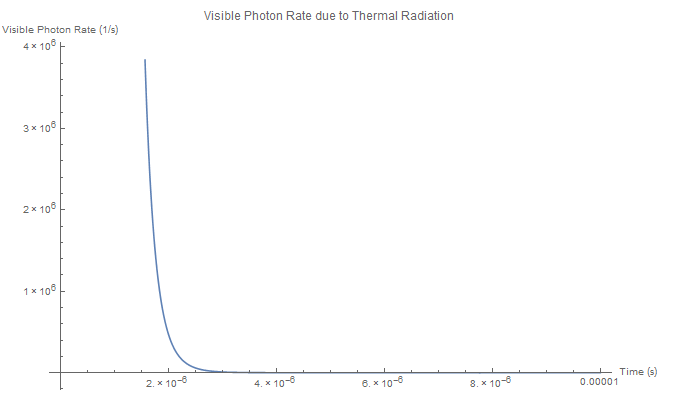
\includegraphics[scale=0.5]{figures/PhotonRateTi.PDF}
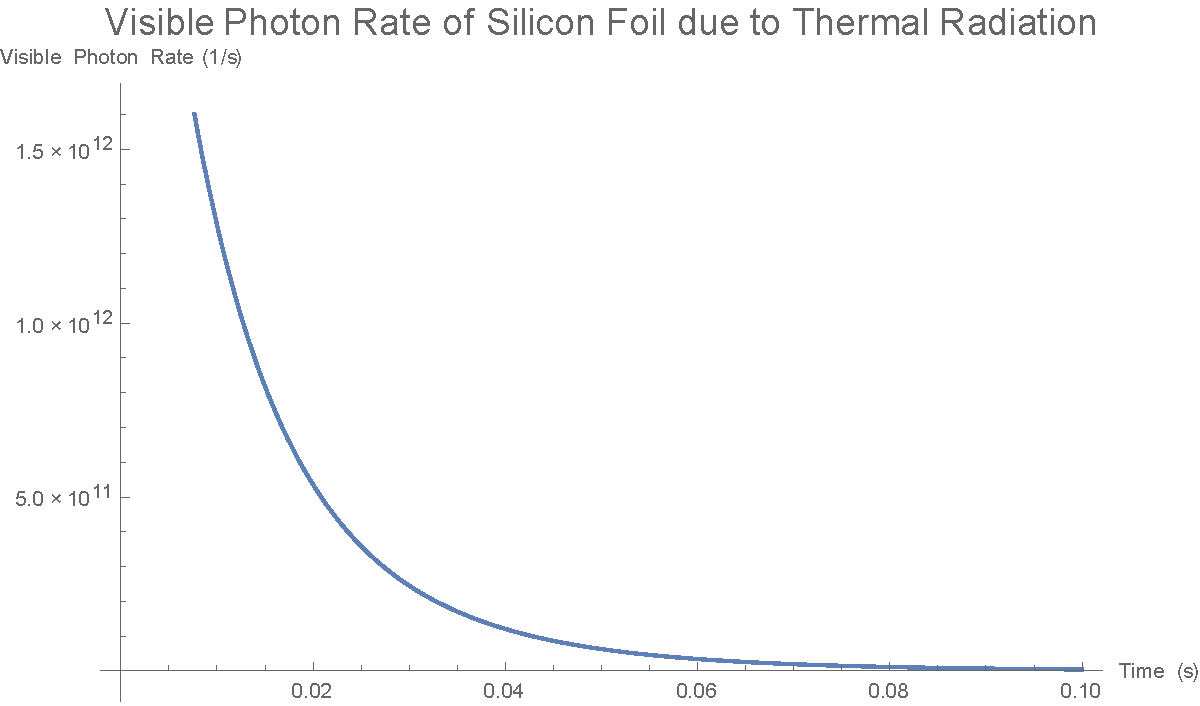
\includegraphics[scale=0.5]{figures/PhotonRateSi.PDF}
\caption{This figure shows the visible photon rate due to thermal radiation emitted from foil as a function of time for both titanium (a) and silicon (b). This neglects effects due to conduction.}
\end{center}
\end{figure}

\begin{figure}
\begin{center}
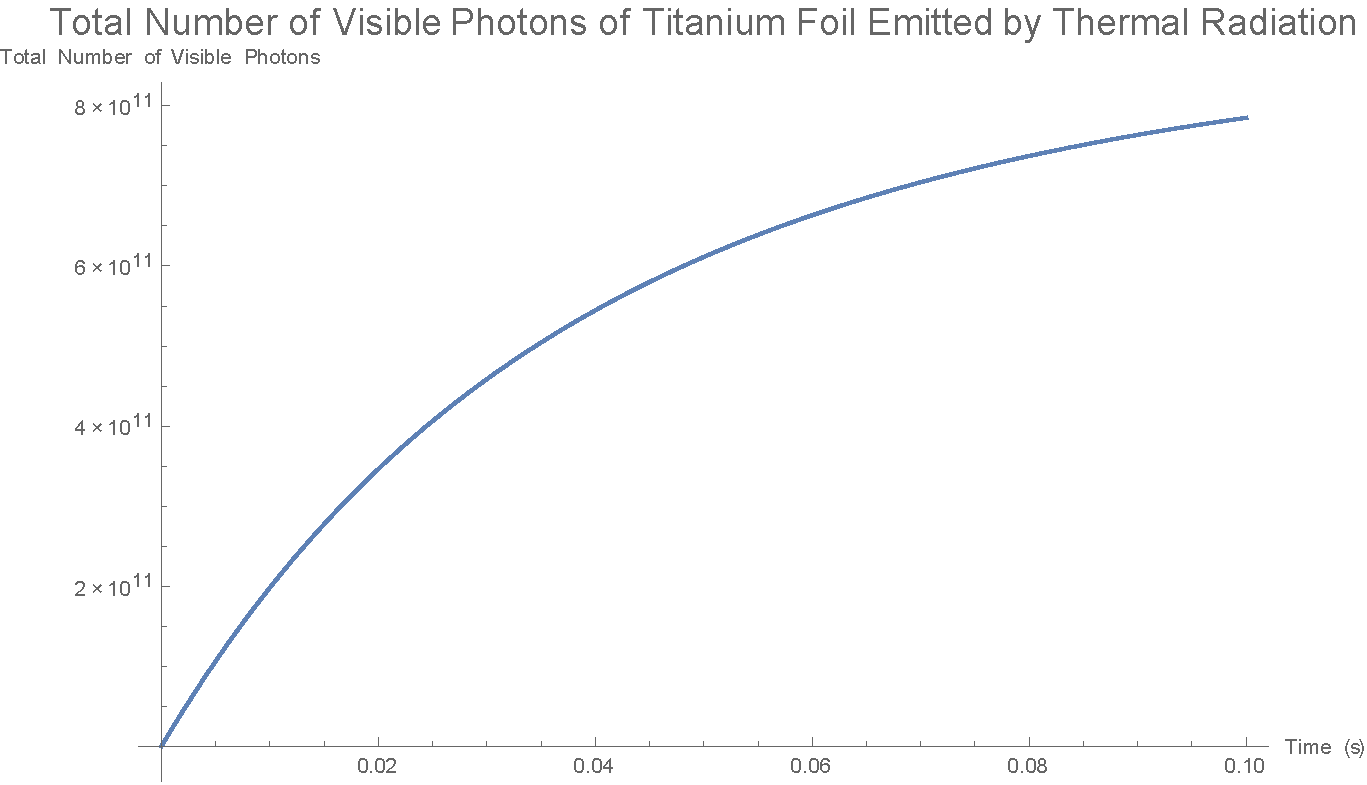
\includegraphics[scale=0.5]{figures/PhotonsTotalTi.PDF}
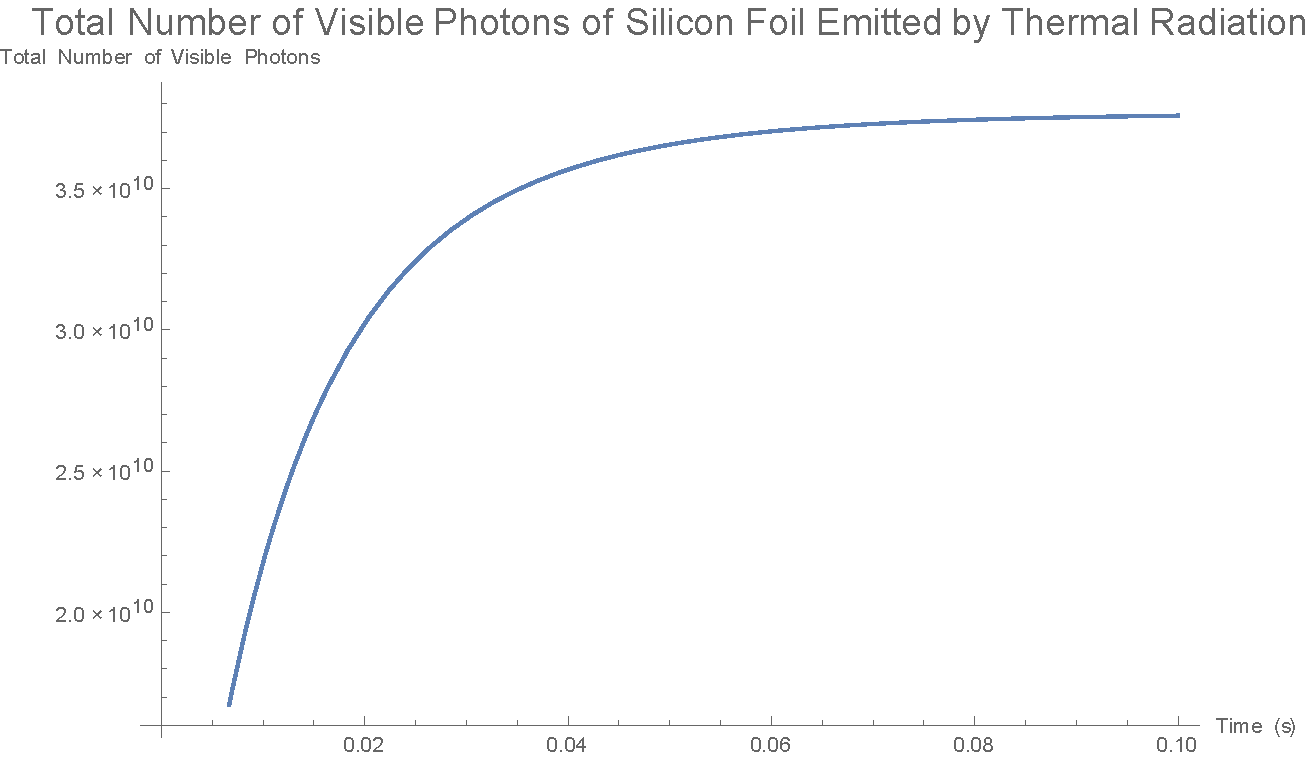
\includegraphics[scale=0.5]{figures/PhotonsTotalSi.PDF}
\caption{This figure shows the total number of visible photons emitted due to thermal radiation at time $t$ from the foil for both titanium (a) and silicon (b). This neglects effects due to conduction.}
\end{center}
\end{figure}

\section*{References}
\begin{enumerate}[{[}1{]}]
\item http://inspirehep.net/record/562218/files/slac-r-576.pdf
\item Accelerator Handbook
\item http://slac.stanford.edu/pubs/slacpubs/15500/slac-pub-15729.pdf
\item http://journals.aps.org/prstab/pdf/10.1103/PhysRevSTAB.10.022802

\end{enumerate}

\end{document}
